    {\large 電気回路 - 磁気 -}
    \begin{multicols}{3}
        \begin{itembox}[l]{磁石と磁界}
            \begin{figure}[H]
                \centering
                \label{fig:magnet}
                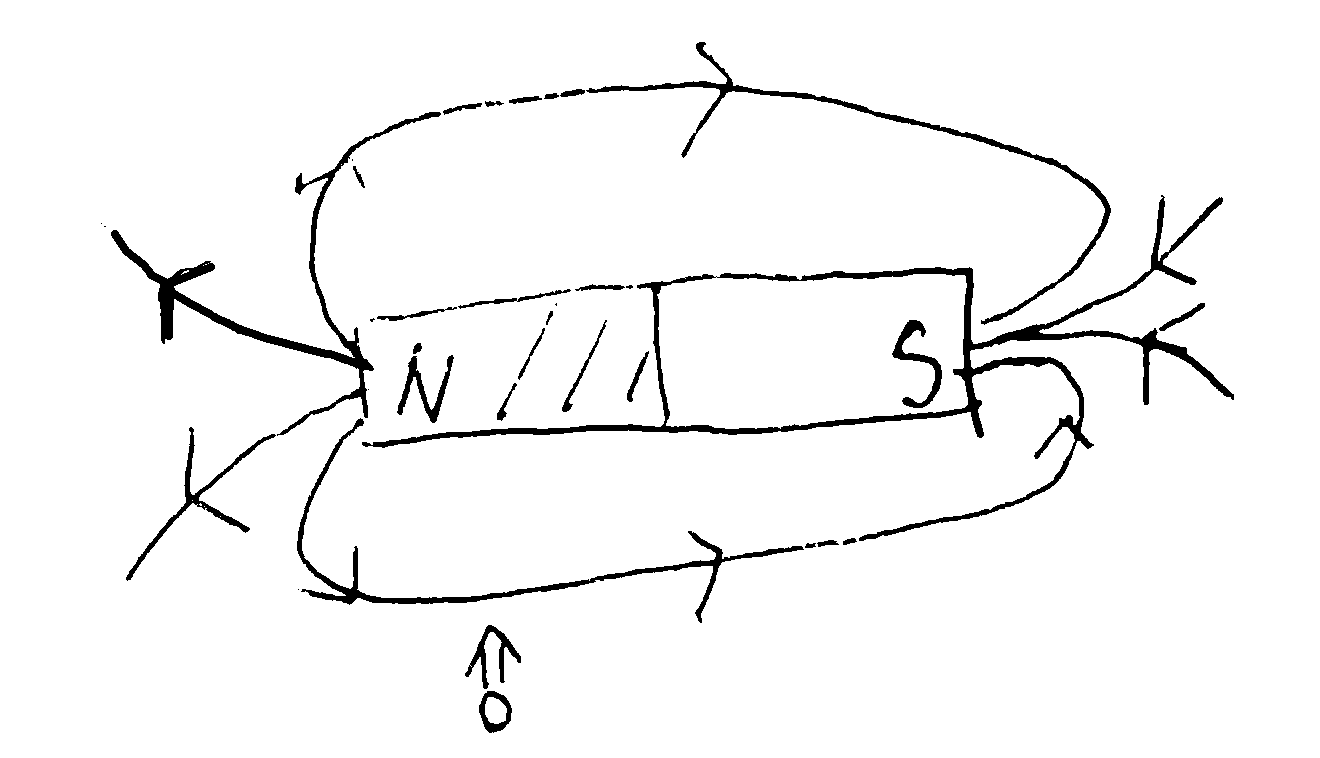
\includegraphics[width=0.7\linewidth]{fig/磁界.png}
                \caption{磁石と磁界}
            \end{figure}
            \begin{itemize}
                \item 磁力線は「N極」=>「S極」へ
                \item 磁力線のある空間を磁界、磁場という
                \item 磁力線同士は交わらない
            \end{itemize}
            \begin{figure}[H]
                \centering
                \label{fig:引力}
                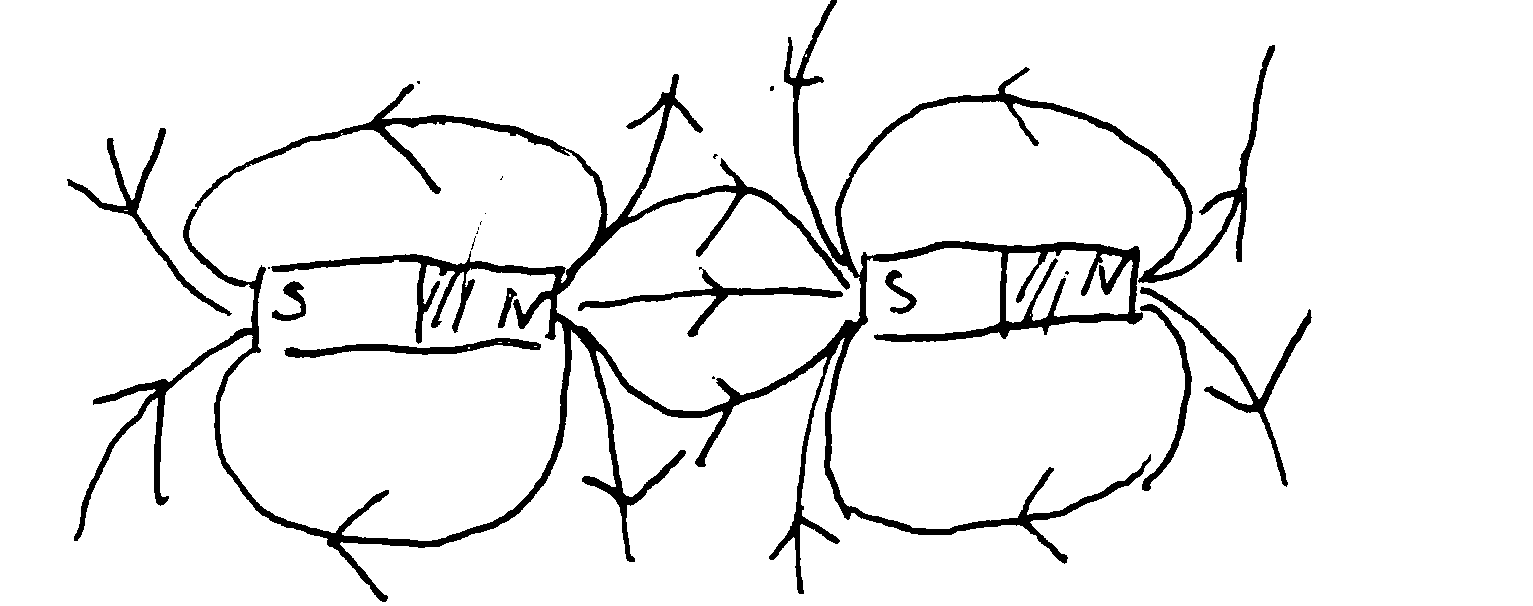
\includegraphics[width=0.7\linewidth]{fig/引力.png}
                \caption{異なる磁極同士に働く引力}
            \end{figure}
            \begin{figure}[H]
                \centering
                \label{fig:斥力}
                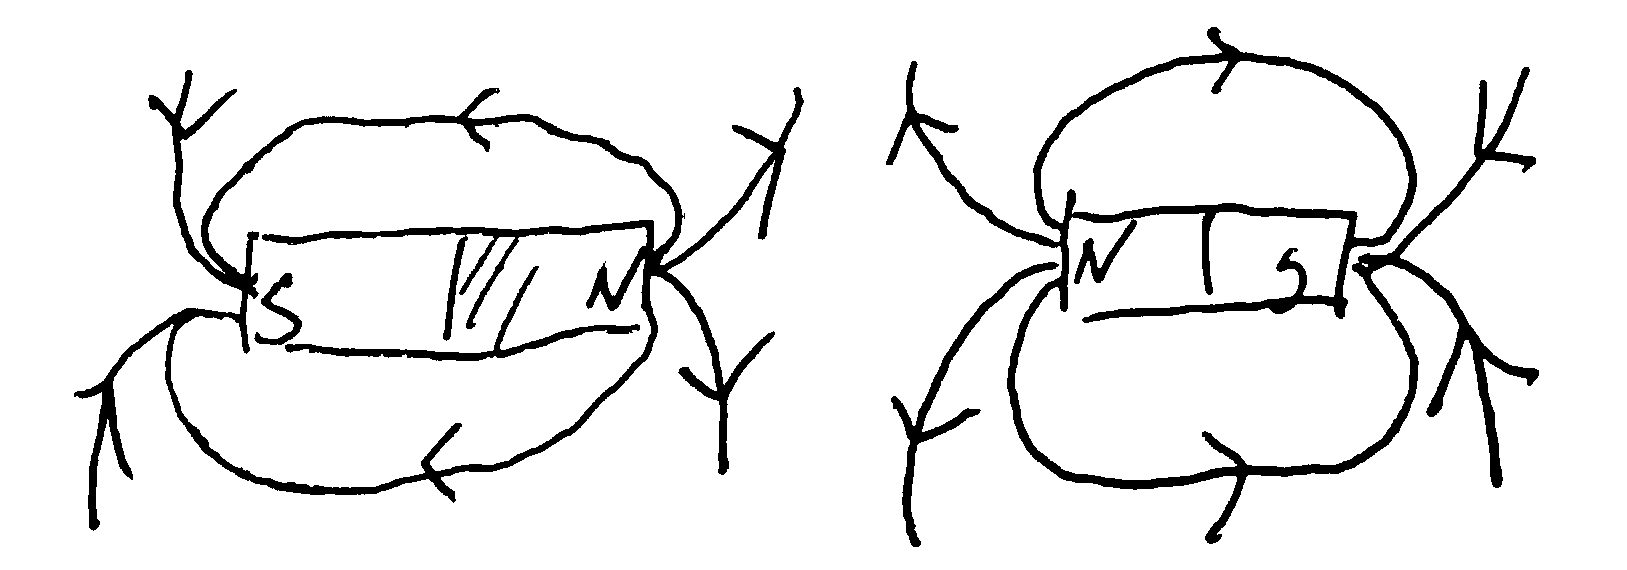
\includegraphics[width=0.7\linewidth]{fig/斥力.png}
                \caption{同じ磁極同士に働く斥力}
            \end{figure}
        \end{itembox}

        \begin{itembox}[l]{電磁石}
            \begin{figure}[H]
                \centering
                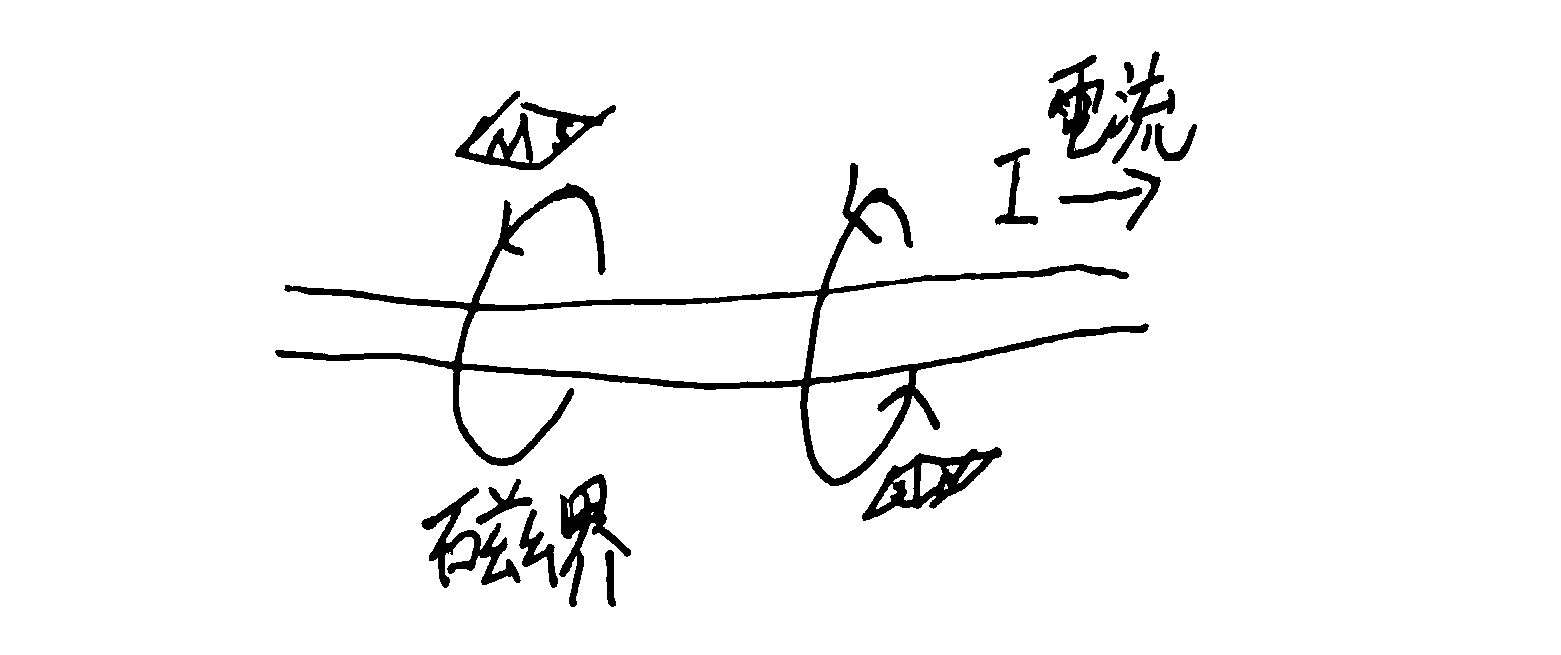
\includegraphics[width=0.6\linewidth]{fig/電線と磁界.png}
                \caption{電流の周囲にできる磁界}
                \label{fig:current_magnet}
            \end{figure}
            \begin{itemize}
                \item 電流が流れると磁界ができる
                \item 磁界の強さは電流の強さに比例する
            \end{itemize}
            \begin{figure}[H]
                \centering
                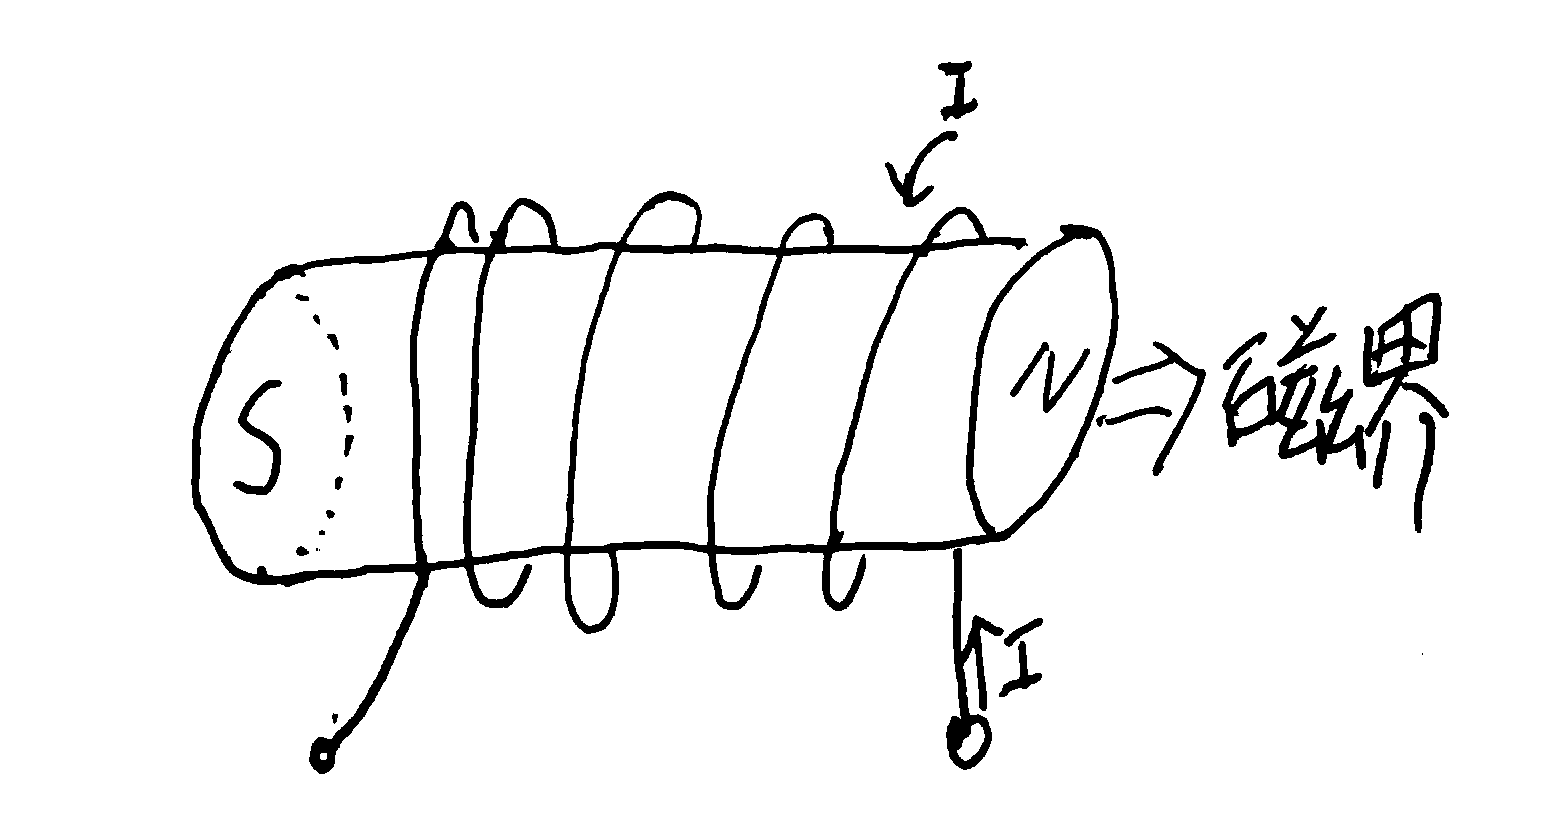
\includegraphics[width=0.6\linewidth]{fig/コイルと磁界.png}
                \caption{コイルの周囲にできる磁界}
                \label{fig:coil_magnet}
            \end{figure}
            \begin{itemize}
                \item 芯(コア)に電線を巻きつける
                \item $n$: 磁界の強さは巻き数の密度に比例
                \item $\mu$:  透磁率の高い材料を芯に使うと磁界が強くなる
                \newline 例:鉄、ニッケル、コバルト
            \end{itemize}
            \begin{align}
                    B &= \mu NI
            \end{align}
        \end{itembox}

        \begin{itembox}[l]{右ねじの法則}
            図\ref{fig:current_magnet}や図\ref{fig:coil_magnet}のように、電流の向きと磁界の向きは右ねじの法則の関係にある。
            右手の親指を電流の向きにしたとき、他の指が巻きつく向きが磁界の向きになる。
        \end{itembox}

        \begin{itembox}[l]{フレミングの左手の法則}
            \begin{figure}[H]
                \begin{minipage}[t]{0.48\linewidth}
                    \centering
                    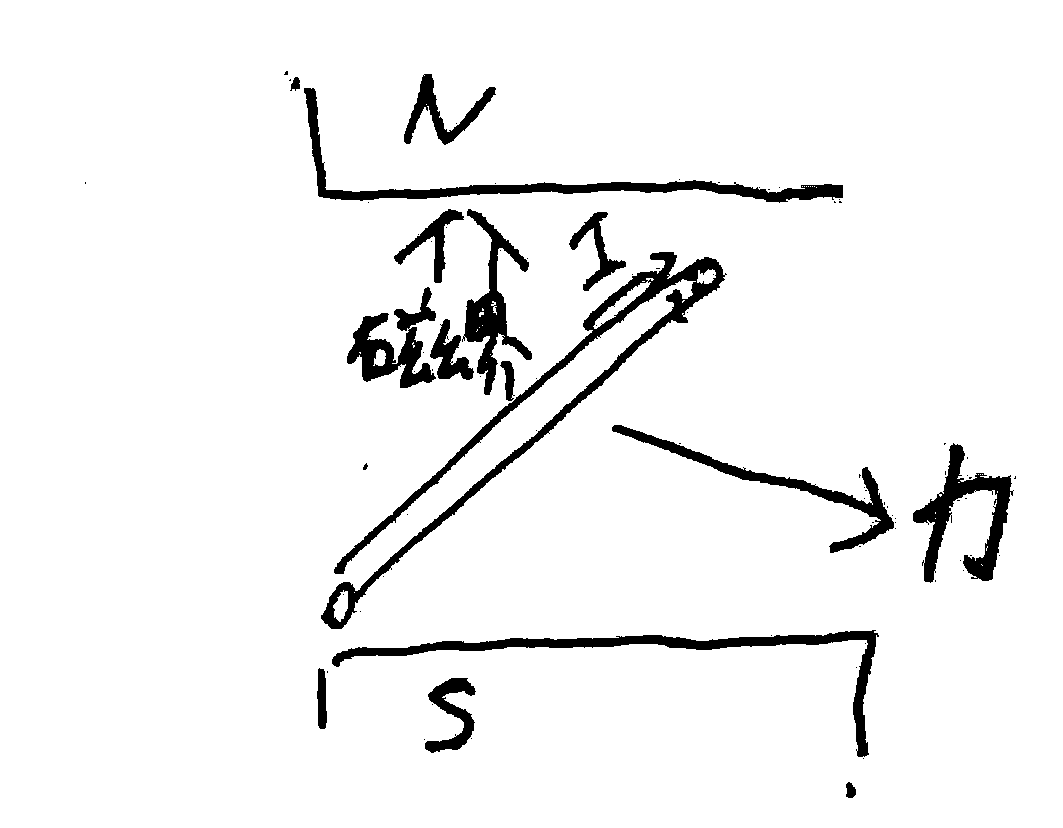
\includegraphics[width=1\linewidth]{fig/アンペアの力.png}
                    \caption{磁界中の導体に働く力}
                    \label{fig:ampere_force}
                \end{minipage}
                \begin{minipage}[t]{0.48\linewidth}
                    \centering
                    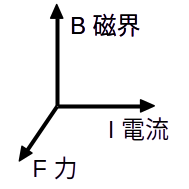
\includegraphics[width=0.8\linewidth]{fig/左手の法則.png}
                    \caption{左手の法則}
                    \label{fig:left_hand}
                \end{minipage}
            \end{figure}
            磁界中の導体に電流が流れると、磁界と電流による磁界の相互作用により導体に力が働く。
            このとき、電流、磁界、力の向きの関係はフレミングの左手の法則と言われる。
            \begin{itemize}
                \item 電流: 左手の中指
                \item 磁界: 左手の人差し指
                \item 力: 左手の親指
            \end{itemize}
            \begin{align}
                \begin{split}
                    F &= BIL\sin\theta\\
                    \varDelta \bm{F}&= I\varDelta \bm{L} \times \bm{B}
                \end{split}
            \end{align}
        \end{itembox}
    \end{multicols}
